%=============================================================================
% ..... THIS IS chapter{RPE-LTP: The full-rate GSM codec } .....
%  ... Revision:
% Nov.1995 - Created <Simao>
% Jan.1996 - Peter Kroon initial revision
% Jan.1996 - RPE description adapted from Peter Kroon's text
% Nov.1996 - William Navarro's comment on GSM history <simao>
% Feb.2000 - Convergence towards STL2000
% Nov.2000 - SG16 Plenary
% Feb.2001 - Edits in example section
%=============================================================================
\chapter{RPE-LTP: The full-rate GSM codec}
%=============================================================================

In 1988, the Groupe Special Mobile of the Conference Europe\'{e}ne
des Postes et Telecommunications (CEPT) approved the first
generation of a pan-European digital cellular radio system operating
at a net rate of 13 kbit/s\footnote{\SF The GSM standard developed
initially under the responsability of the CEPT was later transferred
to the European Standardisation Telecommunications Institute (ETSI),
and the acronym GSM had its meaning changed to Global System for
Mobile Communications. Currently, the GSM specifications are being
maintained by the Third Generation Partnership Project, 3GPP ({\tt
\url{www.3gpp.org}}).}. Its speech coding algorithm, the RPE-LTP
(Regular Pulse Excitation, Long Term Predictor) was a compromise
solution of the two best coders at that stage. The full-rate GSM
system started operation in the beginning of 1992 in some European
countries and its expansion is expected in a mid-term. This coder,
despite not being an ITU-T standard, is relevant for standardization
studies when scenarios involving tandeming conditions between the
PSTN and the European cellular system need to be studied.

The current version of the STL includes a RPE-LTP implementation
based on a  freely available implementation originally produced at
the Technical Institue of the University of Berlin, for a Unix
environment.  This code has been adapted, corrected to work on
several platforms, and tested with the recommended test vectors, all
properly processed.

Details on the algorithm can be found in several references
\cite{RPELTP:BasicConcept,RPELTP:ICASSP88,RPELTP:SpeechCommunication},
besides the Recommendation itself \cite{GSM-06.10}.


\section{Description of the 13 kbit/s RPE-LTP algorithm}
\label{principles}
The RPE-LTP is a frame based coder, encoding 20 ms frames of
input data at a time.
The encoder converts each 160 sample frame (8 kHz sampling rate,
13 bits uniform PCM format) into a bitstream frame of 260 bits.
The decoder uses the 260 bitstream bits to generate
a frame of 160 reconstructed speech samples.


\subsection{RPE-LTP Encoder}
A simplified block diagram of the RPE-LTP encoder \cite{GSM-06.10} is
shown in figure \ref{rpe-encoder}.

%--------------------------------------------------------
% RPE-LTP encoder
%--------------------------------------------------------
\begin{figure}
  \begin{center}
    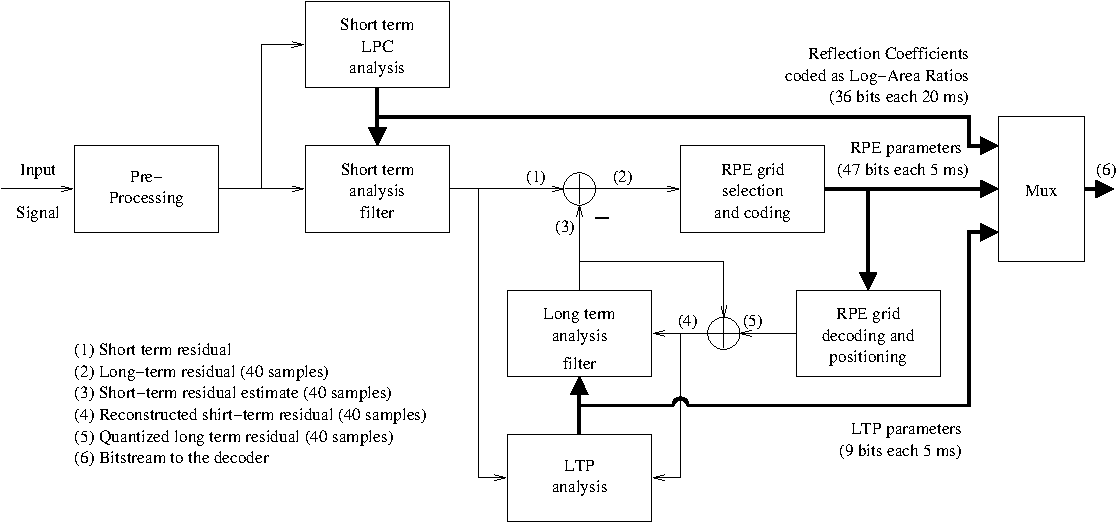
\includegraphics[width=15.5cm]{rpe-enc}
  \end{center}
%%  \begin{center}
%%    \makebox[10cm]{
%%      \rule{0cm}{17.22cm}
%%      \special{psfile=rpe-enc.ps hoffset=-297 voffset=-296 hscale=800 yscale=800}
%%    }
%%  \end{center}
  \caption{Simplified block diagram of the RPE-LTP encoder.
           \label{rpe-encoder}}
\end{figure}
%------------------------------------------------------------

The input speech frame, consisting of 160 uniform 13 bits PCM signal
samples, is first pre-processed to produce an offset-free signal, which
is then subjected to a first-order pre-emphasis filter. The 160
samples obtained are then analyzed to determine the coefficients for
the short-term analysis filter (LPC analysis). Using these coefficients
for the filtering of the same 160 samples produce the 160 samples of
the short-term residual signal. The filter parameters are represented
as reflection coefficients which are transformed to
log-area ratios (LARs) before transmission.

For the following operations, the speech frame is divided into 4
sub-blocks consisting each of 40 samples.
Before the processing of each sub-block, the parameters of the
long-term analysis filter, the LTP lag and the LTP gain, are estimated and
updated in the LTP analysis block. Estimation and update is performed
on the basis of the signal in the current sub-block and a stored
sequence of the 120 previously reconstructed short-term residual
samples.

A block of 40 long-term residual signal samples is obtained by
subtracting 40 estimates of the short-term residual from the
short-term residual signal itself. The resulting block is fed to the Regular
Pulse Excitation (RPE) analysis which performs the basic compression
function.

As a result of the RPE-analysis, the block of 40 input long-term
residual samples is represented by one of 4 candidate sub-sequences
of 13 pulses each. The subsequence selected is identified by the RPE
grid position. The 13 RPE pulses are encoded using Adaptive Pulse
Code Modulation (APCM) with estimation of the sub-block amplitude
which is transmitted to the decoder as side information. The RPE
parameters are also fed to a local RPE decoding and reconstruction
module which produces a block of 40 samples of the quantized version
of the long-term residual signal. By adding these 40 quantized
samples of the long-term residual to the previously obtained block of
short-term residual signal estimates, a reconstructed version of the
current short-term residual signal is obtained. The block of
reconstructed short-term residual signal samples is then fed to the
long-term analysis filter which produces the new block of 40
short-term residual signal estimates to be used for the next
sub-block thereby completing the feedback loop.

\subsection{RPE-LTP Decoder}

The simplified block diagram of the RPE-LTP decoder \cite{GSM-06.10}
is shown in figure \ref{rpe-decoder}.

%--------------------------------------------------------
% RPE-LTP encoder
%--------------------------------------------------------
%Box dimension: 21.17cm x 12.31cm
\begin{figure}
    \begin{center}
        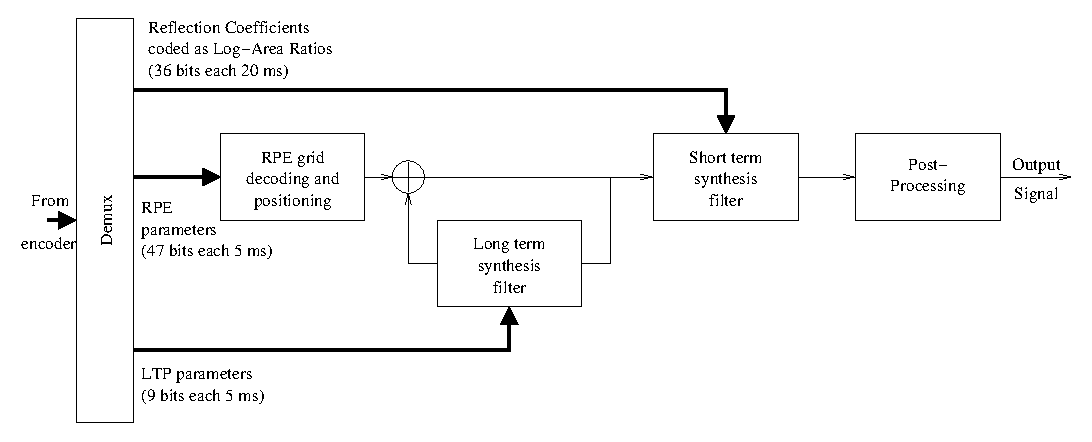
\includegraphics[width=15.5cm]{rpe-dec}
  \end{center}
%%  \begin{center}
%%    \makebox[10cm]{
%%      \rule{0cm}{12.31cm}
%%      \special{psfile=rpe-dec.ps hoffset=-300 voffset=-435}
%%    }
%%  \end{center}
  \caption{Simplified block diagram of the RPE-LTP decoder.
         \label{rpe-decoder}}
\end{figure}
%------------------------------------------------------------

The decoder includes the same structure as the feed-back loop of the
encoder. In error-free transmission, the output of this stage will be
the reconstructed short-term residual samples. These samples are then
applied to the short-term synthesis filter followed by the de-emphasis
filter resulting in the reconstructed speech signal samples.


\section{Implementation}

This implementation of the RPE-LTP algorithm is composed  of several
source files. The interface routines are in {\tt rpeltp.c},  with
prototypes in {\tt rpeltp.h}.

Originally written to be a device driver in Unix (known as {\em
toast}), its interface was adapted  to the specifications of the ITU-T
STL, and modified to operate correctly in a variety  of platforms,
like VAX, IBM PC compatibles, and Unix workstations (Sun and HP).

The problem of storing the state variables was solved by defining a
structure containing all the necessary variables, defining a new type
called {\tt gsm}, which is a pointer to a structure.  By means of
this approach, several streams may be processed in parallel, provided
that one structure is assigned (and that one call to the
encoding/decoding routines is done) for each data stream (this can be
advantageous for machines with support for parallel processing). The
RPE-LTP state structure has the following fields (all except {\em
L\_z2} and {\em mp}  are {\tt short}, which are {\tt long} and {\tt
int}, respectively):
\begin{quote} \normalsize
 {\em dp0} \hfill \pbox{120mm}{Memory of 280 past samples}
 {\em z1} \hfill \pbox{120mm}{DC-offset removal filter memory}
 {\em L\_z2} \hfill \pbox{120mm}{DC-offset removal filter parameter.}
 {\em mp} \hfill \pbox{120mm}{Preemphasis}
 {\em u} \hfill \pbox{120mm}{Eighth-order short term LPC analysis
        coefficients}
 {\em LARpp}\hfill \pbox{120mm}{Log Area Ratio array}
 {\em j}\hfill \pbox{120mm}{Index}
 {\em nrp} \hfill \pbox{120mm}{Long-term synthesis parameter}
 {\em v} \hfill \pbox{120mm}{Ninth order short-term synthesis vector}
 {\em msr} \hfill \pbox{120mm}{Post-processing parameter}
 {\em verbose} \hfill \pbox{120mm}{Flag used only if compiled
                                         with NDEBUG==0}
 {\em fast} \hfill \pbox{120mm}{Enables fast but inaccurate computation.
                                        Does not properly process the test
                                        sequences with this mode turned on.}
\end{quote}

Table \ref{RPE:bitstream} presents the RPE-LTP encoder output
parameters in order of occurence, with parameters defined in
\cite{GSM-06.10}. It should be noted that the bitstream file generated
by the STL implementation of the RPE-LTP algorithm uses an unpacked
format, as other codecs in the STL. Therefore, each of the 76
parameters indicated in table \ref{RPE:bitstream} occupy an unsigned,
right-adjusted 16-bit word. Unlikely to the G.711 and G.726
algorithms, however, the number of significant bits per bitstream
parameter is not the same for all the parameters, as can be seen from
the table. An important implication is that the STL bit error
insertion routines cannot be applied directly to the bitstream
generated by the STL RPE-LTP encoder. This limitation is not a
function of the EID module itself, but of the serialization and
parallelization (S/P) routines {\tt serialize\_*} and {\tt
parallize\_*} implemented in the Utility module, which are able only to
handle bitstreams that have the same number of valid bits per
sample. Solution to this problem still needs to be implemented in the
STL. It should be noted however that, since the full-rate GSM channel
coding is not implemented in the STL, bit error insertion directly in
the unprotected RPE-LTP bitstream will generally not be used. Should
the user need bit error insertion in the unprotected RPE-LTP
bitstream, there are two possible solutions:
\begin{itemize}
  \item it will be necessary to pack the bits for each parameter in
    such a way that, as seen by the S/P routines, each sample in the
    packed bitstream will have a constant number of valid bits per
    bitstream sample. Since there are 260 ($4 \times 5 \times 13$)
    bits for each frame, possible combinations are packed
    bitstreams with 65 16-bit words, of which the lower 4 bits are
    meaningful, or with 20 16-bit words, of which the lower 13 bits are
    meaningful. The former is preferred, despite the longer files
    generated.
  \item the user may modify the demonstration program to generate or accept
    (depending on whether it is an encoding or decoding operation) a
    serial bitstream format, as understood by the EID module, instead
    of a parallel bitstream format.
\end{itemize}

%--------------------------------------------------------------------------
% Table with description of the RPE-LTP bitstream
%--------------------------------------------------------------------------
\begin{table}
\centering\small
\caption{RPE-LTP bitstream format for each 20 ms speech frame.}
\begin{tabular}{|c|c|c|} \hline
\bf Parameter     & \bf Parameter & \bf Number \\
                  & \bf Number    & \bf of Bits\\
\hline
LAR1              &1    & 6 \\
LAR2              &2    & 6 \\
LAR3              &3    & 5 \\
LAR4              &4    & 5 \\
LAR5              &5    & 4 \\
LAR6              &6    & 4 \\
LAR7              &7    & 3 \\
LAR8              &8    & 3 \\
\hline
\multicolumn{3}{|c|}{\bf Sub-frame No. 1} \\
\hline
LTP lag           &9    & 7 \\
LTP gain          &10   & 2 \\
RPE grid position &11   & 2 \\
Block amplitude   &12   & 6 \\
RPE-pulse no. 1   &13   & 3 \\
$\ldots$          &$\ldots$ &$\ldots$\\
RPE-pulse no. 13  &25   & 3 \\
\hline
\multicolumn{3}{|c|}{\bf Sub-frame No. 2} \\
\hline
LTP lag           &26   & 7 \\
LTP gain          &27   & 2 \\
RPE grid position &28   & 2 \\
Block amplitude   &29   & 6 \\
RPE-pulse no. 1   &30   & 3 \\
$\ldots$          &$\ldots$ &$\ldots$\\
RPE-pulse no. 13  &42   & 3 \\
\hline
\multicolumn{3}{|c|}{\bf Sub-frame No. 3} \\
\hline
LTP lag           &43   & 7 \\
LTP gain          &44   & 2 \\
RPE grid position &45   & 2 \\
Block amplitude   &46   & 6 \\
RPE-pulse no. 1   &47   & 3 \\
$\ldots$          &$\ldots$ &$\ldots$\\
RPE-pulse no. 13  &59   & 3 \\
\hline
\multicolumn{3}{|c|}{\bf Sub-frame No. 4} \\
\hline
LTP lag           &60   & 7 \\
LTP gain          &61   & 2 \\
RPE grid position &62   & 2 \\
Block amplitude   &63   & 6 \\
RPE-pulse no. 1   &64   & 3 \\
$\ldots$          &$\ldots$ &$\ldots$\\
RPE-pulse no. 13  &76   & 3 \\
\hline
\end{tabular}
\label{RPE:bitstream}
\end{table}

From the users' perspective, the encoding function is {\tt
rpeltp\_encode}, and the decoding function is {\tt rpeltp\_decode}.
Before using these functions, the state variable for either the
encoder or the decoder must be initialized by {\tt rpeltp\_init}. It
should be noted that encoder and decoder need individual state
variables to work properly. After all the processing is performed, the
memory allocated for the state variables can be freed by calling {\tt
rpeltp\_delete}. The following sub-sections describe these four entry
functions for the STL RPE-LTP module.

\subsection{{\tt rpeltp\_encode}} \label{sec:rpeencode}

{\bf Syntax: }

{\tt
\#include "rpeltp.h"\\
void rpeltp\_encode (\ttpbox{110mm}{
            gsm {\em rpe\_state}, short {\em *inp\_buf},
            short {\em *rpe\_frame});
         }
}

{\bf Prototype: }    rpeltp.h

{\bf Description: }

        Simulation of the GSM full-rate RPE-LTP encoder. The 16-bit,
        left-justified linear-PCM input array of \short samples {\em
        inp\_buf} are processed by the RPE-LTP encoder and the encoded
        bit-stream is returned in the right-justified array of \short
        samples {\em rpe\_frame}, with one sample for each encoded
        parameter. The input frame has 160 samples and the encoded
        frame has 76 samples.

        The state variables are saved in the structure pointed by {\em
        rpe\_state}, previously initialized by a call to {\tt
        rpeltp\_init()}. The reset can be stablished by making a call
        to {\tt rpeltp\_init()}.

{\bf Variables: }
\begin{Descr}{\DescrLen}
\item[\pbox{20mm}{\em rpe\_state}] %\rulex{1mm}\\
               A pointer to the state variable structure. All the
               variables here are for internal use of the RPE-LTP
               algorithm and should not be changed by the
               user. Fields of this structure are described above.

\item[\pbox{20mm}{\em inp\_buf}] %\rulex{1mm}\\
               Is the linear-PCM input sample buffer which must have 160
               left-justified 16-bit linear-PCM \short samples. Only
               the 13 MSb are used.

\item[\pbox{20mm}{\em rpe\_frame}] %\rulex{1mm}\\
               Is the encoded sample buffer. Each \short sample will
               contain the encoded parameters as right-justified
               samples. The actual number of significant bits per
               sample will depend on each parameter.
\end{Descr}

        {\bf Return value: }        None.


\subsection{{\tt rpeltp\_decode}} \label{sec:rpedecode}

{\bf Syntax: }

{\tt
\#include "rpeltp.h"\\
void rpeltp\_decode (\ttpbox{110mm}{
            gsm {\em rpe\_state}, short {\em *rpe\_frame},
            short {\em *out\_buf});
         }
}

{\bf Prototype: }    rpeltp.h

{\bf Description: }

        Simulation of the GSM full-rate RPE-LTP decoder. The encoded
        bit-stream in the input array of right-justified \short
        samples {\em rpe\_frame} is used to reconstruct a block of the
        speech signal using the RPE-LTP decoder. The reconstructed
        speech block is returned in the 16-bit, left-justified
        linear-PCM output array of \short samples {\em inp\_buf}. The
        input frame has 76 samples and the decoded frame has 160
        samples.

        The state variables are saved in the structure pointed by {\em
        rpe\_state}, previously initialized by a call to {\tt
        rpeltp\_init()}. The reset can be established by calling {\tt
        rpeltp\_init()}.

{\bf Variables: }
\begin{Descr}{\DescrLen}
\item[\pbox{20mm}{\em rpe\_state}] %\rulex{1mm}\\
               A pointer to the state variable structure. All the
               variables here are for internal use of the RPE-LTP
               algorithm and should not be changed by the user. Fields
               of this structure are described above.

\item[\pbox{20mm}{\em rpe\_frame}] %\rulex{1mm}\\
               Is the encoded sample buffer, which must have 76
               right-justified \short samples. The actual number of
               bits per sample will depend on each parameter.

\item[\pbox{20mm}{\em out\_buf}] %\rulex{1mm}\\
               Is the output samples buffer, which will contain 160
               left-justified, 13-bit linear-PCM \short samples. The
               three LSbs are set to zero.
\end{Descr}

        {\bf Return value: }        None.

\subsection{{\tt rpeltp\_init}}

{\bf Syntax: }

{\tt
\#include "rpeltp.h"\\
gsm rpeltp\_init (void);
}

{\bf Prototype: }    rpeltp.h

{\bf Description: }

        Initializes the state variables for the RPE-LTP encoder or decoder.
        Combined coder and decoder operation requires a different state
        variable for the encoding and the decodeing part.

{\bf Variables: } None.

{\bf Return value: }

A pointer to an initialized state variable structure defined by the type
{\tt gsm}. Returns NULL in case of failure.

\subsection{{\tt rpeltp\_delete}}

{\bf Syntax: }

{\tt
\#include "rpeltp.h"\\
void rpeltp\_init (gsm rpe\_state);
}

{\bf Prototype: }    rpeltp.h

{\bf Description: }

Releases memory allocated to a state variable previously
initialized by rpeltp\_init().

{\bf Variables: }
\begin{Descr}{\DescrLen}
\item[\pbox{20mm}{\em rpe\_state}] %\rulex{1mm}\\
        A pointer to a previously initialized RPE-LTP state variable
        structure.
\end{Descr}

{\bf Return value: }

None.


\section{Portability and compliance}

The portability test for these routines has been done using
the test sequences designed by the GSM for the RPE-LTP
(available from ETSI), which were also used to verify the compliance of
the encoding and decoding function to the full-rate GSM voice codec
Recommendation \cite[Annex C]{GSM-06.10}.

This routine has been tested in VAX/VMS with VAX-C and gcc, in the PC
with Borland C v3.0 (16-bit mode) and gcc (32-bit mode). In the Unix
environment in a Sun workstation with cc, acc, and gcc, and in HP with
gcc. In all tested cases, 100\% of the test sequences passed when the
following symbols were defined at compilation time: {\tt SASR}, {\tt
USE\_FLOAT\_MUL} and {\tt NDEBUG}. The symbol {\em FAST} must not be
defined for perfomance compliant with the GSM 06.10 Recommendation,
while {\tt USE\_FLOAT\_MUL} {\bf must} be defined at compilation
time. The symbol {\tt NeedFunctionPrototypes} must be undefined for
pre-ANSI-C compilers (e.g. SunOS cc compiler).


%-----------------------------------------------------------------
\section{Example code}

%.................................................................
\subsection {Description of the demonstration program}

One program is provided as demonstration program for the RPE-LTP module,
rpedemo.c.

Program {\tt rpedemo.c} accepts input files in either 16-bit linear
PCM format, 16-bit, right-justified A-law format, or 16-bit,
right-justified $\mu$-law format for the encoding operation. The
output of the decoder can also be in any of these formats, but it will
have the same format as the encoding operation if encoding and
decoding is performed in a single pass (default). If the encoding and
decoding operations are performed in separate steps, the format of the
output signal does not need to match the format of the original linear
PCM signal.  The encoder output and decoder input are signals in
16-bit, right-justified samples, as described before in Sections
\ref{sec:rpeencode} and \ref{sec:rpedecode}. Three operations are
possible: encode and decode in a single pass (default), encode-only
(option {\em -enc}), or decode-only (option {\em -dec}).

%..........................................................................
\subsection {Simple example}

The following C code gives an example of RPE-LTP coding and decoding
using as input 13-bit, linear-PCM speech samples, which are encoded
and decoded at 13 kbit/s.

{\tt\small
\begin{verbatim}
#include <stdio.h>
#include "ugstdemo.h"
#include "rpeltp.h"

#define BLK_LEN 160

int main(argc, argv)
  int       argc;
  char     *argv[];
{
  gsm       encoder_state, decoder_state;

  char      FileIn[180], FileOut[180];
  short     bs_buf[BLK_LEN], inp_buf[BLK_LEN], out_buf[BLK_LEN];
  FILE     *Fi, *Fo;

  /* Get parameters for processing */
  GET_PAR_S(1, "_Input File: .................. ", FileIn);
  GET_PAR_S(2, "_Output File: ................. ", FileOut);

  /* Initialize state structures */
  encoder_state = rpeltp_init();
  decoder_state = rpeltp_init();

  /* Opening input and output LOG-PCM files */
  Fi = fopen(FileIn, RB);
  Fo = fopen(FileOut, WB);

 /* File processing */
  reset = 1;                    /* set reset flag as YES */
  while (fread(inp_buf, BLK_LEN, sizeof(short), Fi) == BLK_LEN)
  {
    /* Encode input linear PCM samples */
    rpeltp_encode(encoder_state, inp_buf, bs_buf, BLK_LEN);

    /* Decode samples */
    rpeltp_decode(decoder_state, bs_buf, out_buf);

    /* Write decoded samples */
    fwrite(out_buf, BLK_LEN, sizeof(short), Fo);

    if (reset)
      reset = 0;                /* set reset flag as NOMORE */
  }

  /* Free memory */
  rpe_delete(decoder_state);
  rpe_delete(encoder_state);

  /* Close input and output files */
  fclose(Fi);
  fclose(Fo);
  return 0;
}
\end{verbatim}
}
